\Chapter{\textit{Design} de Testes Economicamente Viáveis}

\cite{Sandi} afirma que escrever código que muda é uma arte a qual a prática depende de três habilidades diferentes.

Primeiro, você precisa entender \textit{design} orientado a objetos. Código com \textit{design} pobre é naturalmente difícil de alterar. De um ponto de vista prático, a capacidade de alteração é a única métrica de \textit{design} que importa; código que é fácil de mudar tem um bom \textit{design}. Se você chegou até aqui é justo supor que você já tem uma base pela qual começar a praticar a escrita de código fácil de alterar.

Segundo, você deve ser habilidoso em refatoração de código. Não no sentido casual de "vá até a sua aplicação e tire algumas coisas", mas no sentido real, maduro, à prova de balas definido por Martin Fowler no livro \textit{Refactoring: Improving the Design of Existing Code}\cite{Fowler1999}:

\say{Refatoração é o processo de mudar um sistema de software de um modo que não altere o comportamento externo do código, mas melhore a estrutura interna.}

Repare na parte \textit{não altere o comportamento externo do código}. Refatorar, em sua definição formal, não adiciona novo comportamento, ele melhora a estrutura existente. É um processo preciso que altera código via passos muito pequenos, cuidadosos, incrementais que infalivelmente transforma um \textit{design} em outro.

Bom \textit{design} preserva flexibilidade máxima no menor custo ao adiar decisões a cada oportunidade. Postergando qualquer comprometimento até que requerimentos mais específicos cheguem. Quando esse dia chegar, será através da refatoração que você vai transformar a estrutura atual do código em uma que acomodará os novos requerimentos. Novas \textit{features} serão adicionadas apenas depois que tiver refatorado o código com sucesso.

Se as suas habilidades de refotrar são fracas, melhore-as. A necessidade de refactoring contínuo é uma consequência natural do bom \textit{design}; seus esforços para melhorar o \textit{design} irão dar seu maior retorno apenas quando você refatorar com facilidade.

Para finalizar, a arte de escrever código mutável requer a habilidade de escrever testes que tenham valor. Testes te dão confiança para refatorar constantemente. Testes eficientes provam que o código alterado continua se comportando corretamente sem aumentar os custos no geral. Bons testes são escritos de uma forma que a alteração do código não force a reescrita dos testes, permitindo que refatorações possam ser realizadas sem medo e insegurança.

A escrita de testes que executem este truque é um questão de \textit{design} e é o tópico desse capítulo.

Uma compreensão de \textit{design} orientado a objetos, boas habilidades de refatoração e a habilidade de escrever testes eficientes formam a base principal onde reside o código de alteração fácil.

Código com bom \textit{design} é fácil de alterar, \textit{refactoring} é como você muda de um \textit{design} para o próxima e testes te libertam para refatorar de forma impune. 

\section{Testando Intencionalmente}

Os argumentos mais comuns a favor de se ter testes é o de que eles reduzem \textit{bugs}, fornecem documentação e que escrever testes primeiro melhora o \textit{design} da aplicação.

Esses benefícios, apesar de válidos, são representações para um objetivo mais profundo. O verdadeiro propósito de testar, assim como o verdadeiro propósito do \textit{design}, é a redução de custos. Se escrever, manter e executar testes consome mais tempo do que seria necessário para corrigir \textit{bugs}, escrever documentação e fazer o \textit{design} de aplicações, testes claramente não valem a pena serem escritos e nenhuma pessoa racional iria contradizer isso.

É comum para programadores que são novos em testes encontrarem-se em um estado infeliz onde os testes que eles escrevem custam mais do que o valor que esses testes promovem, e quem assim sendo querem discutir sobre o valor de se testar. Esses são programadores os quais acreditam serem altamente produtivos em suas formas sem testes, pois são os mesmos que bateram na parede to testar primeiro e tropeçaram até parar. Suas tentativas em programação com testes primeiro resultaram em menos entregas, e o desejo de retornar a serem produtivos fizeram com que eles retornassem aos antigos hábitos e esquecessem a escrita de testes.

A solução para o problema de testes custosos, no entanto, não é parar de testar, mas se tornar melhor nisso ao invés. Obter um bom retorno dos testes requer clareza de intenção e saber o que, quando e como testar.

\section{Conhecendo as suas Intenções}

Testar tem muito benefícios em potencial, alguns óbvios, outros mais obscuros. Uma compreensão completa desses benefícios vai aumentar a sua motivação para alcança-los.

\subsection{Encontrando \textit{bugs}}

Encontrar falhas, ou \textit{bugs}, cedo no processo de desenvolvimento rendem grandes dividendos. Não apenas é mais fácil encontrar e corrigir um \textit{bug} quanto mais próximo da sua época de criação, mas conseguir o código certo mais cedo do que mais tarde pode ter um efeito positivo não esperado no \textit{design} resultante.

Saber que você pode (ou não pode) fazer algo mais cedo talvez façam você escolher alternativas no dia presente que alteram as opções de \textit{design} disponíveis no futuro. Além disso, conforme o código se acumula, \textit{bugs} incorporados acumulam dependências. Corrigir esses \textit{bugs} mais tarde no processo pode necessitar da mudança de muito código com dependências. Corrigir esses \textit{bugs} mais cedo sempre custa menos.

\subsection{Fornecimento de Documentação}

Testes providenciam a única documentação confiável de \textit{design}. A história que eles contam permanecem verdadeiras muito tempo depois que a documentos em papel se tornam obsoletos e a memória humana falha. Escreva seus testes como se você esperasse que o seu futuro eu tenha amnésia. Lembre-se que você vai esquecer; escreva testes que te lembrem da história que uma vez você viveu. 

\subsection{Adiando Decisões de \textit{Design}}

Testes permitem que você adie de forma segura decisões de \textit{design}. Conforme as suas habilidades de \textit{design} melhoram você vai começar a escrever aplicações que estão semeadas com lugares onde você sabe que o \textit{design} precisa de alguma coisa, mas você não tem ainda informações suficientes para saber exatamente o que. Esses são os lugares onde você está aguardando informações adicionais, resistindo de forma valente as forças que obrigam você a se cometer a um \textit{design} específico.

Esses pontos de decisão ''pendente'' são frequentemente codificados como \textit{hacks} concretos levemente embaraçosos escondidos atrás de interfaces totalmente apresentáveis. Essa situação ocorre quando você está ciente de um caso concreto no presente, mas você espera totalmente que novos casos chegarão em um futuro próximo. Você sabe que em algum ponto você vai estar melhor servido por código que controla melhor esses muitos casos concretos em uma única abstração, mas exatamente agora você não tem informação suficiente para antecipar qual será essa abstração.

Quando seus testes dependem de interfaces você pode refatorar o código por baixo com total desapego. Os testes verificam a continuação do bom comportamento da interface e mudanças no código subjacente não forçam a reescrita dos testes. Depender intencionalmente em interfaces permite que você use testes para postergar decisões de \textit{design} com segurança e sem penalidade alguma.  

\subsection{Suporte para Abstrações}

Quando mais informações finalmente chegarem e você tomar a próxima decisão de \textit{design}, você vai alterar o código de maneiras que aumentem seu nível de abstração. Onde mora outros benefícios de testes no \textit{design}.

Bom \textit{design} naturalmente progride em direção a pequenos objetos independentes que dependem de abstrações. O comportamento de aplicações com bom \textit{design} gradualmente são o resultado de interações entre essas abstrações. Abstrações são componentes de \textit{design} maravilhosamente flexíveis, mas as melhorias que eles fornecem vêm com um pequeno custo: Enquanto cada abstração possa ser fácil de entender individualmente, não há um único local no código que torne óbvio o comportamento do todo.

Conforme a base de código cresce e o número de abstrações aumenta, testes se tornam cada vez mais necessários. Há um nível de abstração em \textit{design} onde é quase impossível fazer qualquer alteração de forma segura a menos que o código tenha testes. Testes são os registros das interfaces de cada abstração e como tal eles são a sua proteção. Eles permitem que você adie decisões de \textit{design} e crie abstrações em qualquer nível de profundidade útil.

\subsection{Expondo Falhas de \textit{Design}}

O próximo benefício de testes é que eles expõem falhas de \textit{design} no código subjacente. Se um teste requer um configuração trabalhosa, o código espera muito contexto. Se testar um objeto traz um monte de outros objetos, o código tem muitas dependências. Se o teste é difícil de escrever, outro objetos irão achar difícil reutilizar o código. 

Quando o \textit{design} é ruim, testar é difícil. No entanto, não é garantido que o inverso seja verdade. Testes custosos não necessariamente significam que a aplicação tem \textit{design} pobre. É tecnicamente possível escrever testes ruins para código com bom \textit{design}. Assim sendo, para testes diminuírem seus custos, tanto a aplicação subjacente e os testes precisam ter bom \textit{design}.

Seu objetivo é ganhar todos os benefícios dos testes pelo menor custo possível. O melhor jeito de alcançar esse objetivo é escrever testes fracamente acoplados apenas sobre as coisas que importam.

\section{Sabendo o que Testar}

A maioria dos programadores escrevem testes demais. Isso não é sempre óbvio porque em muitos casos o custo desses testes desnecessários são tão altos que os programadores envolvidos já desistiram de testar completamente. Não é que eles não têm testes. Eles têm uma grande, mas obsoleta suíte de testes, que nunca roda. Um jeito simples de obter melhores utilidades dos testes é escrever menos deles. O jeito mais seguro de conseguir isso é testar tudo apenas uma vez e no lugar certo. 

Remover duplicação de testes diminui o custo da mudança de testes quando há mudanças na aplicação, e colocar testes nos lugares certos garantem que eles serão forçados a mudar apenas quando absolutamente necessário. Refinar seus testes para apenas o essencial requer ter uma ideia muito clara sobre o que você pretende testar, uma que pode ser derivada de princípios de \textit{design} que você já conhece.

Pense em uma aplicação orientada a objetos como uma série de mensagens passando entre um conjunto de caixas pretas. Lidar com cada objeto como se fosse uma caixa preta restringe o que outros tem permissão para saber e limita o conhecimento público sobre qualquer mensagens que atravessam suas fronteiras.

Objetos com bom \textit{design} têm fronteiras que são fortes. Cada um é como a cápsula espacial exibida na Figura \ref{img:origem_mensagens}. Nada no exterior pode ver dentro, nada dentro pode ver o exterior e apenas algumas mensagens explicitamente acordadas podem passar pelas fechaduras.

\begin{figure}[!htbp]
  \center
  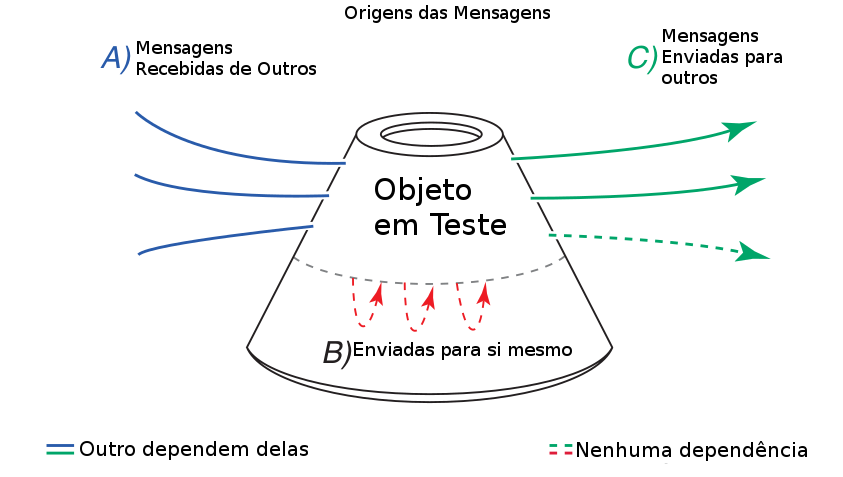
\includegraphics[scale=0.40]{imagens/origem_mensagens.png}
  \caption{Objetos em teste são como cápsulas espaciais, mensagens abrem suas brechas}
  \label{img:origem_mensagens}
\end{figure}

Essa ignorância da parte interna de todos os outros objetos é a parte central do \textit{design}. Lidar com objetos como se eles fossem apenas e exatamente as mensagens as quais eles respondem permite que você faça o \textit{design} de uma aplicação que é alterável, e é o seu entendimento sobre a importância dessa perspectiva que vai permitir que você crie testes que fornecem o máximo de benefício com o mínimo de custo.

Os princípios de \textit{design} que você está impondo a sua aplicação também se aplicam aos seus testes. Cada teste é meramente outro objeto da aplicação que precisa usar uma classe existente. Quanto mais o teste fica acoplado aquela classe, mais emaranhado os dois se tornam e mais vulnerável o teste se torna a ser forçado a mudar desnecessariamente.

Não apenas você deveria limitar o acoplamento, mas os poucos que você permite deveriam ser a coisas estáveis. A coisa mais estável sobre qualquer objeto é a sua interface pública; segue-se logicamente que os testes que você escreve devem ser para mensagens que são definidas nas interfaces públicas. Os testes mais custosos e inúteis são aqueles que abrem um buraco nas paredes de contenção de um objeto ao se acoplarem a detalhes internos instáveis. Esses testes ansiosos provam nada sobre exatidão no geral de uma aplicação, mas no entanto aumentam custos porque eles quebram a cada refatoração da classe por baixo.

Testes deveriam se concentrar nas mensagens de entrada e saída que cruzam as fronteiras do objeto. As mensagens de entrada compõem a interface pública do objeto que recebe. As mensagens de saída, por definição, são entradas para outros objetos e então são parte da interface de algum outro objeto, como ilustrado na Figura \ref{img:dependencia}.

\begin{figure}[!htbp]
  \center
  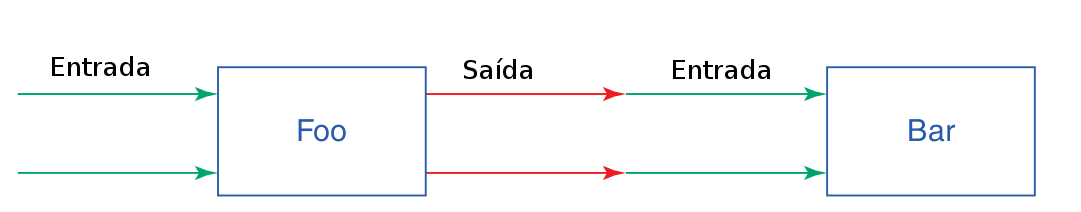
\includegraphics[scale=0.40]{imagens/dependencia.png}
  \caption{Uma mensagem de saída de um objeto é a mensagem de entrada de outro objeto}
  \label{img:dependencia}
\end{figure}

Na Figura \ref{img:dependencia}, mensagens que são entrada em Foo compõem a interface pública de Foo. Foo é responsável por testar sua própria interface e faz isso ao fazer afirmações (\textit{assertions}) sobre os resultados que essas mensagens retornam. Testes que fazem afirmações sobre os valores que as mensagens retornam são testes de \textit{estado}. Testes assim comumente afirmam que os resultados retornados por uma mensagem são iguais a um valor esperado.

A Figura \ref{img:dependencia} também mostra Foo enviando mensagens para Bar. Uma mensagem enviada de Foo para Bar é uma mensagem de saída para Foo, mas uma mensagem de entrada para Bar. Essa mensagem é parte da interface pública de Bar e portanto todos os testes de estado devem então estarem confinados em Bar. Foo não precisa, nem deve, testar o estado dessas mensagens de saída. A regra geral é que objetos devem fazer afirmações sobre o estado apenas das mensagens de suas próprias interfaces públicas. Seguir essa regra limita os testes de retorno de valores de mensagens a apenas um lugar e remove duplicações desnecessárias, fazendo com que seus testes fiquem DRY (\textit{Don't Repeat Yourself}) e reduzindo custos de manutenção.

O fato de você não precisar testar o estado de mensagens de saída não significa que mensagens de saída não precisam de teste algum. Existem dois sabores de mensagens de saída, e um deles requer um tipo diferente de teste.

Algumas mensagens de saída não têm efeito colateral e portanto importam apenas para quem as envia. Quem envia a mensagem com certeza se importa com o resultado que obtém como retorno (por que outro motivo enviar uma mensagem?), mas nenhuma outra parte da aplicação se importa se a mensagem é enviada. Mensagens de saída como essa são conhecidas como \textit{queries} (consultas) e elas não precisam ser testadas pelo objeto que envia a mensagem. Mensagens de consulta são parte da interface pública do objeto que as recebe, o qual já implementa todos os testes de estado necessários.

Contudo, muitas mensagens de saída têm efeitos colaterais (um arquivo é escrito, um registro no banco de dados é salvado, uma ação é tomada por um observador) sobre os quais sua aplicação depende. Essas mensagens são comandos e é responsabilidade do objeto que as envia provar que essas mensagens estão sendo enviadas de forma apropriada. Provar que uma mensagem é enviada é um teste de comportamento, não estado, e envolve afirmações sobre o número de vezes, e com quais argumentos, a mensagem é enviada.

Aqui, então, estão as diretrizes sobre o que testar: Mensagens de entrada devem ser testadas pelo estado que retornam. Mensagens de comando de saída devem ser testadas para certificar que elas são enviadas. Mensagens de saída de consulta não devem ser testadas.

Enquanto os objetos da sua aplicação lidem uns com os outros estritamente via interface pública, seus testes não precisam saber de nada mais. Quando você testa esse conjunto mínimo de mensagens, nenhuma mudança no comportamento privado de qualquer objeto pode afetar nenhum teste. Quando você testa mensagens de comando de saída apenas para provar que elas são enviadas, seus testes fracamente acoplados podem tolerar mudanças na aplicação sem serem forçados a mudar por sua vez. Enquanto as interfaces públicas permanecerem estáveis, você pode escrever testes uma vez e eles irão manter você seguro para sempre.

\section{Sabendo Quando Testar}

Você deve escrever testes primeiro, sempre que faça sentido fazer isso dessa forma.

Infelizmente, julgar quando isso faz sentido pode ser um desafio para \textit{designers} novatos, o que torna esse conselho menos do que útil. Novatos frequentemente escrevem código que é muito acoplado; eles combinam responsabilidades sem relação e vinculam muitas dependências em todos os objetos. Suas aplicações são tapeçarias bem tecidas de código emaranhado onde nenhum objeto vive em isolação. É muito difícil de testar essas aplicações retroativamente porque testes são reuso e esse código não pode ser reutilizado.

Escrever testes primeiro força que um mínimo de reutilização seja construído no objeto durante seu princípio; seria impossível de outra forma escrever qualquer teste. Assim sendo, \textit{designers} novatos são melhores servidos escrevendo código de testes primeiro. A falta de habilidade de \textit{design} deles talvez torne isso desconcertantemente difícil, mas se eles persistirem eles terão pelo menos código testável, algo que de outra forma não seria verdade.

Esteja avisado, no entanto, que escrever testes primeiro não é substituto para e não garante uma aplicação com bom \textit{design}. A reusabilidade que resulta dos testes primeiro é uma melhoria em relação a nenhum teste, mas a aplicação resultante ainda pode cair longe de ter bom \textit{design}. Novatos bem intencionados frequentemente escrevem testes caros e duplicados ao redor de código fortemente acoplado e bagunçado. É uma verdade lamentável que o código mais complexo é geralmente escrito pela pessoa menos qualificada. Isso não reflete uma complexidade natural da tarefa por baixo, mas uma falta de experiência por parte do programador ao invés. Programadores novatos ainda não têm as habilidades para escrever código simples.

As aplicações super complicadas que estes novatos produzem deveriam ser vistas como triunfos da perseverança; é um milagre que essas aplicações funcionem no fim das contas. O código é difícil. As aplicações são difíceis de mudar e cada refatoração quebra todos os testes. Esse custo alto de mudança pode facilmente iniciar um queda de produtividade que pode desanimar todos os interessados. Mudanças desencadeiam efeitos colaterais em cascata ao longo da aplicação, e o custo de manutenção dos testes fazem com que eles pareçam custosos em relação ao valor deles.

Se você é um novato nessa situação, é importante manter a confiança no valor dos testes. Realizada no tempo certo e na quantidade certa, testar, e escrever código de testes primeiro, irá diminuir seus custos no geral. Ganhar esses benefícios requer a aplicação dos princípios de \textit{design} orientado a objetos em todos os lugares, tanto no código da aplicação quanto no código dos seus testes. Seu conhecimento recém-descoberto de \textit{design} já torna mais fácil escrever código testável, a maior parte do restante desse capítulo ilustra como aplicar esses princípios de \textit{design} durante a construção de testes. Pela razão de aplicações com bom \textit{design} serem fáceis de mudar, e teste com bom \textit{design} possivelmente evitarem mudança completamente, essas melhorias de \textit{design} no geral pagam tudo dramaticamente.

\textit{Designers} experientes colhem melhorias mais sutis da escrita de testes primeiro. Não é que eles não conseguem se beneficiar com isso ou que eles nunca vão descobrir algo inesperado ao seguir o que isso dita, em vez disso os ganhos acumulados da reutilização forçada de código são aqueles que eles já possuem. Esses programadores já escrevem código reutilizável fracamente acoplado; testes adicionam valores de outras formas.

Não é inédito para \textit{designers} experientes explorarem soluções para um problema, ou seja, escrever códigos que são apenas experimentos. Esses experimentos são exploratórios, para soluções incertas de alguns problemas. Uma vez que a clareza é obtida e o \textit{design} se sugere, esses programadores então regressam para a escrita de código de produção com testes primeiro.

Seu objetivo geral é a criação de aplicações com bom \textit{design} que possuem cobertura de testes aceitáveis. O melhor jeito de alcançar essa meta varia de acordo com a experiência e pontos fortes do programador.

Essa licença para usar o seu próprio julgamento não é uma permissão para pular os testes. Código com \textit{design} pobre sem testes é apenas código legado que não pode ser testado. Não superestime seus pontos fortes e use um visão inflada de si mesmo como desculpas para evitar testes. Enquanto algumas vezes faz sentido escrever um pouco de código da maneira antiga, você deveria errar ao lado de testes primeiro.

\section{Sabendo Como Testar}

Qualquer um pode criar um novo \textit{framework} de testes em Ruby e algumas vezes parece que todo mundo já criou. O brilhante \textit{framework} novo pode conter uma \textit{feature} que você simplesmente não pode viver sem; se você entende os custos e benefícios, sinta-se livre para escolher qualquer \textit{framework} que sirva para você.

